\chapter{Desenvolvimento}

\section{Definição do Produto e Fluido Refrigerante}

Para o desenvolvimento do projeto, definiu-se como produto a ser refrigerado o pescado fresco, recebido na câmara de refrigeração a \textit{0°C} e armazenado em temperatura de conservação de \textit{-25°C}, condição típica para armazenamento comercial de longo prazo. As propriedades termofísicas do produto, incluindo calor específico, densidade e calor latente de congelamento, bem como as temperaturas de operação, encontram-se especificadas em \cite{calor_especifico_II} e \cite{costa1982refrigeracao}.

A seleção do fluido refrigerante considerou critérios técnicos, econômicos e ambientais. O refrigerante R-134a (1,1,1,2-tetrafluoretano) foi escolhido por apresentar características adequadas à faixa de temperatura requerida, baixo custo relativo, ampla disponibilidade no mercado e extensa utilização em aplicações de refrigeração comercial. Adicionalmente, o R-134a possui potencial de destruição da camada de ozônio (ODP) nulo, embora apresente potencial de aquecimento global (GWP) moderado de 1430, sendo considerado um fluido de transição aceitável para esta aplicação.

As propriedades termodinâmicas do R-134a, incluindo entalpia, entropia, temperatura e pressão em diferentes estados do ciclo, foram determinadas através da biblioteca CoolProp, uma base de dados de código aberto amplamente validada. A integração com rotinas computacionais desenvolvidas em Python permitiu o cálculo automatizado dos ciclos de refrigeração e a análise paramétrica do sistema.

\section{Estimativa da Carga Térmica de Refrigeração}

A seleção adequada do compressor requer inicialmente a determinação da carga térmica do sistema, que corresponde à taxa de calor a ser removida do produto durante o processo de resfriamento. Para este projeto, considerou-se uma câmara de refrigeração com capacidade volumétrica de 200 litros, operando com fator de ocupação de 70\%, o que resulta em uma massa de pescado de aproximadamente 136 kg, conforme a Equação~\ref{massa peixe}.

\begin{equation}
    m_{\text{peixe}} = \rho \cdot V_{\text{útil}}
    \label{massa peixe}
\end{equation}

O tempo de \textit{pull-down}, isto é, o período necessário para reduzir a temperatura do produto desde a condição inicial (0°C) até a temperatura de armazenamento (-25°C), foi especificado em 8 horas. Este parâmetro é crítico para o dimensionamento, pois define a potência mínima de refrigeração necessária. A carga térmica sensível foi calculada pela Equação~\ref{Q resfriamento}, considerando apenas a remoção de calor sensível do pescado, sem contemplar a fase de congelamento.

\begin{equation}
    \dot{Q}_{\text{produto}} = \frac{m \cdot c \cdot \Delta T}{\Delta t}
    \label{Q resfriamento}
\end{equation}

\begin{table}[ht]
\centering
\begin{tabular}{|l|c|c|}
\hline
\textbf{Parâmetro} & \textbf{Símbolo} & \textbf{Valor} \\ \hline
Densidade do pescado & $\rho$ & 972 kg/m³ \\ \hline
Volume útil da câmara & $V_{\text{útil}}$ & 0,14 m³ \\ \hline
Calor específico do pescado & $c$ & 1,71 kJ/(kg·K) \\ \hline
Variação de temperatura & $\Delta T$ & 25 K \\ \hline
Tempo de \textit{pull-down} & $\Delta t$ & $2,88 \times 10^{4}$ s (8 h) \\ \hline
\end{tabular}
\caption{Parâmetros utilizados no cálculo da carga térmica do produto.}
\label{tab:tabela dados}
\end{table}

Substituindo os valores da Tabela~\ref{tab:tabela dados} na Equação~\ref{Q resfriamento}, obtém-se a carga térmica mínima requerida:

\begin{equation}
    \dot{Q}_{\text{produto}} = 202,6~\text{W}
    \label{carga}
\end{equation}

É importante ressaltar que este valor representa apenas a carga térmica do produto. Em um projeto completo, deveriam ser consideradas cargas térmicas adicionais, como infiltração de ar, ganho de calor pelas paredes, iluminação e respiração do produto, que podem aumentar significativamente a carga total do sistema.

\subsection{Seleção de Compressores Candidatos}

Com a carga térmica de referência estabelecida, procedeu-se à seleção de compressores candidatos através da ferramenta \textit{Product Selector} disponibilizada pelo fabricante Embraco. Para aplicações em baixas temperaturas de evaporação, como a especificada neste projeto (-25°C), são recomendados compressores da linha LBP (\textit{Low Back Pressure}), projetados especificamente para trabalhar com elevadas razões de compressão.

\begin{figure}[ht]
    \centering
    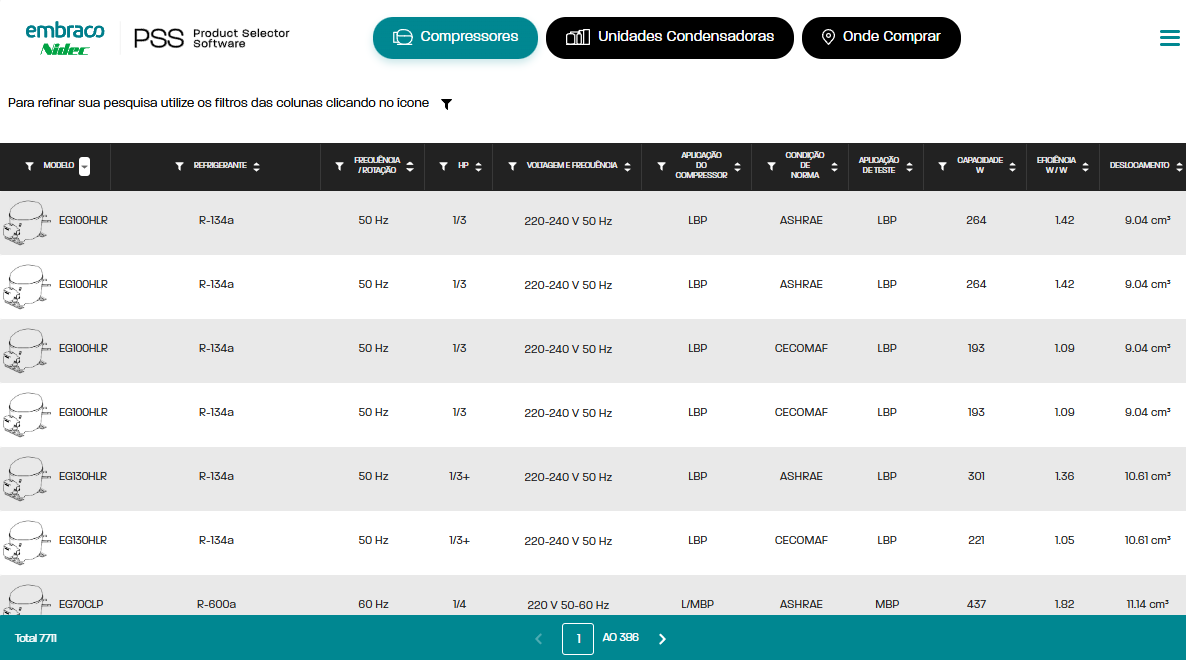
\includegraphics[width=0.8\linewidth]{Imagens/Desenvolvimento/PSS-embraco.png}
    \caption{Interface do seletor de produtos Embraco utilizado para pré-seleção dos compressores.}
    \label{fig:seletor de produtos}
\end{figure}

Os catálogos técnicos dos compressores pré-selecionados fornecem dados de desempenho obtidos em condições padronizadas de teste, incluindo temperaturas de evaporação e condensação, capacidade de refrigeração, consumo de potência elétrica e corrente nominal. Estes dados permitem uma análise comparativa detalhada do desempenho termodinâmico e econômico de cada modelo.

Foram selecionados quatro modelos de compressores herméticos que atendem aos requisitos de capacidade de refrigeração, apresentados na Tabela~\ref{tab:compressores escolhidos}.

\begin{table}[ht]
\centering
\begin{tabular}{|l|c|c|}
\hline
\textbf{Modelo} & \textbf{Potência Nominal [W]} & \textbf{Custo Estimado [R\$]} \\ \hline
EGAS80HLR & 240 & 650 \\ \hline
EGZS60HLP & 180 & 1340 \\ \hline
EGZS70HLC & 202 & 1130 \\ \hline
FFU70HAK & 221 & 600 \\ \hline
\end{tabular}
\caption{Compressores pré-selecionados para análise comparativa.}
\label{tab:compressores escolhidos}
\end{table}

\newpage

\section{Ciclo de Refrigeração Ideal}

Como referencial teórico para análise de desempenho, foi inicialmente considerado um ciclo de refrigeração ideal baseado no ciclo de Carnot reverso. Este ciclo representa o limite termodinâmico superior de eficiência para qualquer sistema de refrigeração operando entre duas fontes térmicas a temperaturas especificadas. O ciclo ideal de Carnot para refrigeração é composto por quatro processos reversíveis: compressão isentrópica do vapor saturado, condensação isotérmica à temperatura da fonte quente, expansão isentrópica do líquido saturado e evaporação isotérmica à temperatura da fonte fria, conforme ilustrado na Figura~\ref{fig: ciclo ideal}.

\begin{figure}[ht]
    \centering
    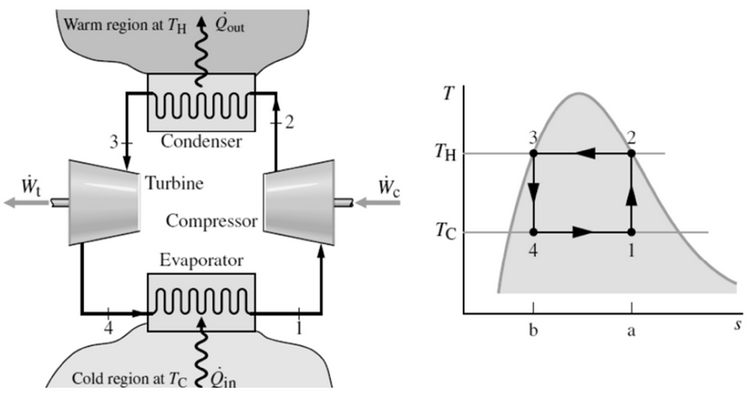
\includegraphics[width=0.6\linewidth]{Imagens/Desenvolvimento/carnot.png}
    \caption{Diagrama temperatura-entropia do ciclo ideal de Carnot para refrigeração.}
    \label{fig: ciclo ideal}
\end{figure}

Para o cálculo do coeficiente de performance (COP) de Carnot, consideraram-se as temperaturas de armazenamento do produto ($T_L = -25$°C = 248 K) e ambiente externo ($T_H = 35$°C = 308 K) como as temperaturas das fontes fria e quente, respectivamente. Esta simplificação representa o cenário termodinâmico mais favorável possível, desconsiderando irreversibilidades inerentes aos processos reais, como perdas por atrito, transferência de calor com diferença finita de temperatura e quedas de pressão.

O COP de Carnot é definido pela relação entre o efeito refrigerante ($\dot{Q}_L$) e o trabalho de compressão ($\dot{W}_c$), podendo ser expresso exclusivamente em função das temperaturas absolutas das fontes térmicas:

\begin{equation}
    \text{COP}_{\text{Carnot}} = \frac{T_L}{T_H - T_L} = \frac{\dot{Q}_L}{\dot{W}_c}
    \label{eq:cop carnot}
\end{equation}

Substituindo os valores de temperatura na Equação~\ref{eq:cop carnot}, obtém-se:

\begin{equation}
    \text{COP}_{\text{Carnot}} = \frac{248}{308 - 248} = 4,13
\end{equation}

A partir do COP de Carnot e da carga térmica determinada anteriormente (Equação~\ref{carga}), pode-se estimar a potência mínima teórica de compressão necessária:

\begin{equation}
    \dot{W}_{c,\text{ideal}} = \frac{\dot{Q}_L}{\text{COP}_{\text{Carnot}}} = \frac{202,6}{4,13} = 49,1~\text{W}
    \label{eq:potencia ideal}
\end{equation}

Este valor representa um limite termodinâmico inferior para a potência de compressão. Na prática, devido às irreversibilidades do ciclo real, à necessidade de diferenças de temperatura finitas nos trocadores de calor e às perdas mecânicas e elétricas do compressor, a potência real requerida será significativamente superior, tipicamente de 2 a 4 vezes maior que o valor ideal calculado.

\section{Ciclo de Refrigeração Real}

A partir dos parâmetros estabelecidos na análise preliminar, desenvolveu-se uma rotina computacional em Python para simular o ciclo de refrigeração por compressão de vapor considerando as não idealidades do processo real. O ciclo implementado segue a configuração apresentada na Figura~\ref{fig:ciclo padrão}, onde o fluido refrigerante R-134a entra no compressor como vapor saturado (estado 2), é comprimido isentropicamente até vapor superaquecido (estado 3), condensa isobaricamente até líquido saturado (estado 4) e sofre expansão isentálpica através de um dispositivo de expansão até a pressão de evaporação (estado 1).

\begin{figure}[ht]
    \centering
    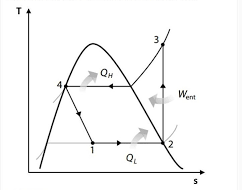
\includegraphics[width=0.6\linewidth]{Imagens/Desenvolvimento/Diagrama.png}
    \caption{Diagrama pressão-entalpia do ciclo real de refrigeração por compressão de vapor.}
    \label{fig:ciclo padrão}
\end{figure}


\subsection{Validação do Modelo com Dados de Catálogo}

Inicialmente, o programa foi validado utilizando as condições de teste padronizadas fornecidas nos catálogos técnicos dos compressores selecionados. Os fabricantes tipicamente apresentam dados de desempenho para combinações específicas de temperaturas de evaporação e condensação, permitindo a verificação da consistência do modelo desenvolvido. Esta etapa foi fundamental para assegurar a confiabilidade dos resultados e identificar quais compressores apresentam capacidade adequada para atender aos requisitos do projeto.

\subsection{Modelagem Termodinâmica do Ciclo}

A modelagem do ciclo real baseia-se na metodologia apresentada por \cite{paper_referencia}, que permite estimar a vazão mássica do refrigerante e a capacidade de refrigeração efetiva do compressor a partir de suas características operacionais. A potência de compressão real é calculada pelo balanço de energia no compressor, considerando a variação de entalpia entre a sucção e descarga:

\begin{equation}
    \dot{W}_c = \dot{m}(h_3 - h_4)
    \label{W compressor}
\end{equation}

\noindent onde $\dot{m}$ é a vazão mássica de refrigerante, $h_3$ é a entalpia específica do vapor saturado na entrada do compressor e $h_4$ é a entalpia específica do vapor superaquecido na saída do compressor, calculada assumindo compressão isentrópica ($s_3 = s_4$) e conhecendo-se a pressão de condensação.

A capacidade de refrigeração do sistema é determinada pelo calor absorvido no evaporador:

\begin{equation}
    \dot{Q}_L = \dot{m}(h_2 - h_1)
    \label{capacidade evaporador}
\end{equation}

O coeficiente de performance do ciclo real é então calculado pela razão entre o efeito refrigerante e o trabalho de compressão:

\begin{equation}
    \text{COP}_{\text{real}} = \frac{\dot{Q}_L}{\dot{W}_c} = \frac{h_1 - h_4}{h_2 - h_1}
    \label{cop real}
\end{equation}

As propriedades termodinâmicas do R-134a em cada estado do ciclo (pressão, temperatura, entalpia e entropia) foram calculadas utilizando a biblioteca CoolProp, que implementa equações de estado de alta precisão. As Figuras \ref{fig:ciclo comp 1} e \ref{fig:ciclo comp 2} demonstram os resultados obtidos.

Para efeito de comparação e quantificação das perdas associadas às irreversibilidades do ciclo real, calculou-se paralelamente o COP do ciclo ideal de Carnot operando entre as mesmas temperaturas das fontes térmicas. A eficiência termodinâmica ou eficiência de segunda lei ($\eta_{II}$) do ciclo real pode então ser expressa como:

\begin{equation}
    \eta_{II} = \frac{\text{COP}_{\text{real}}}{\text{COP}_{\text{Carnot}}}
    \label{eficiencia segunda lei}
\end{equation}


Esta análise permite identificar o potencial de melhoria do sistema e quantificar o impacto das irreversibilidades no desempenho global do ciclo de refrigeração.

\begin{figure}[ht]
    \centering
    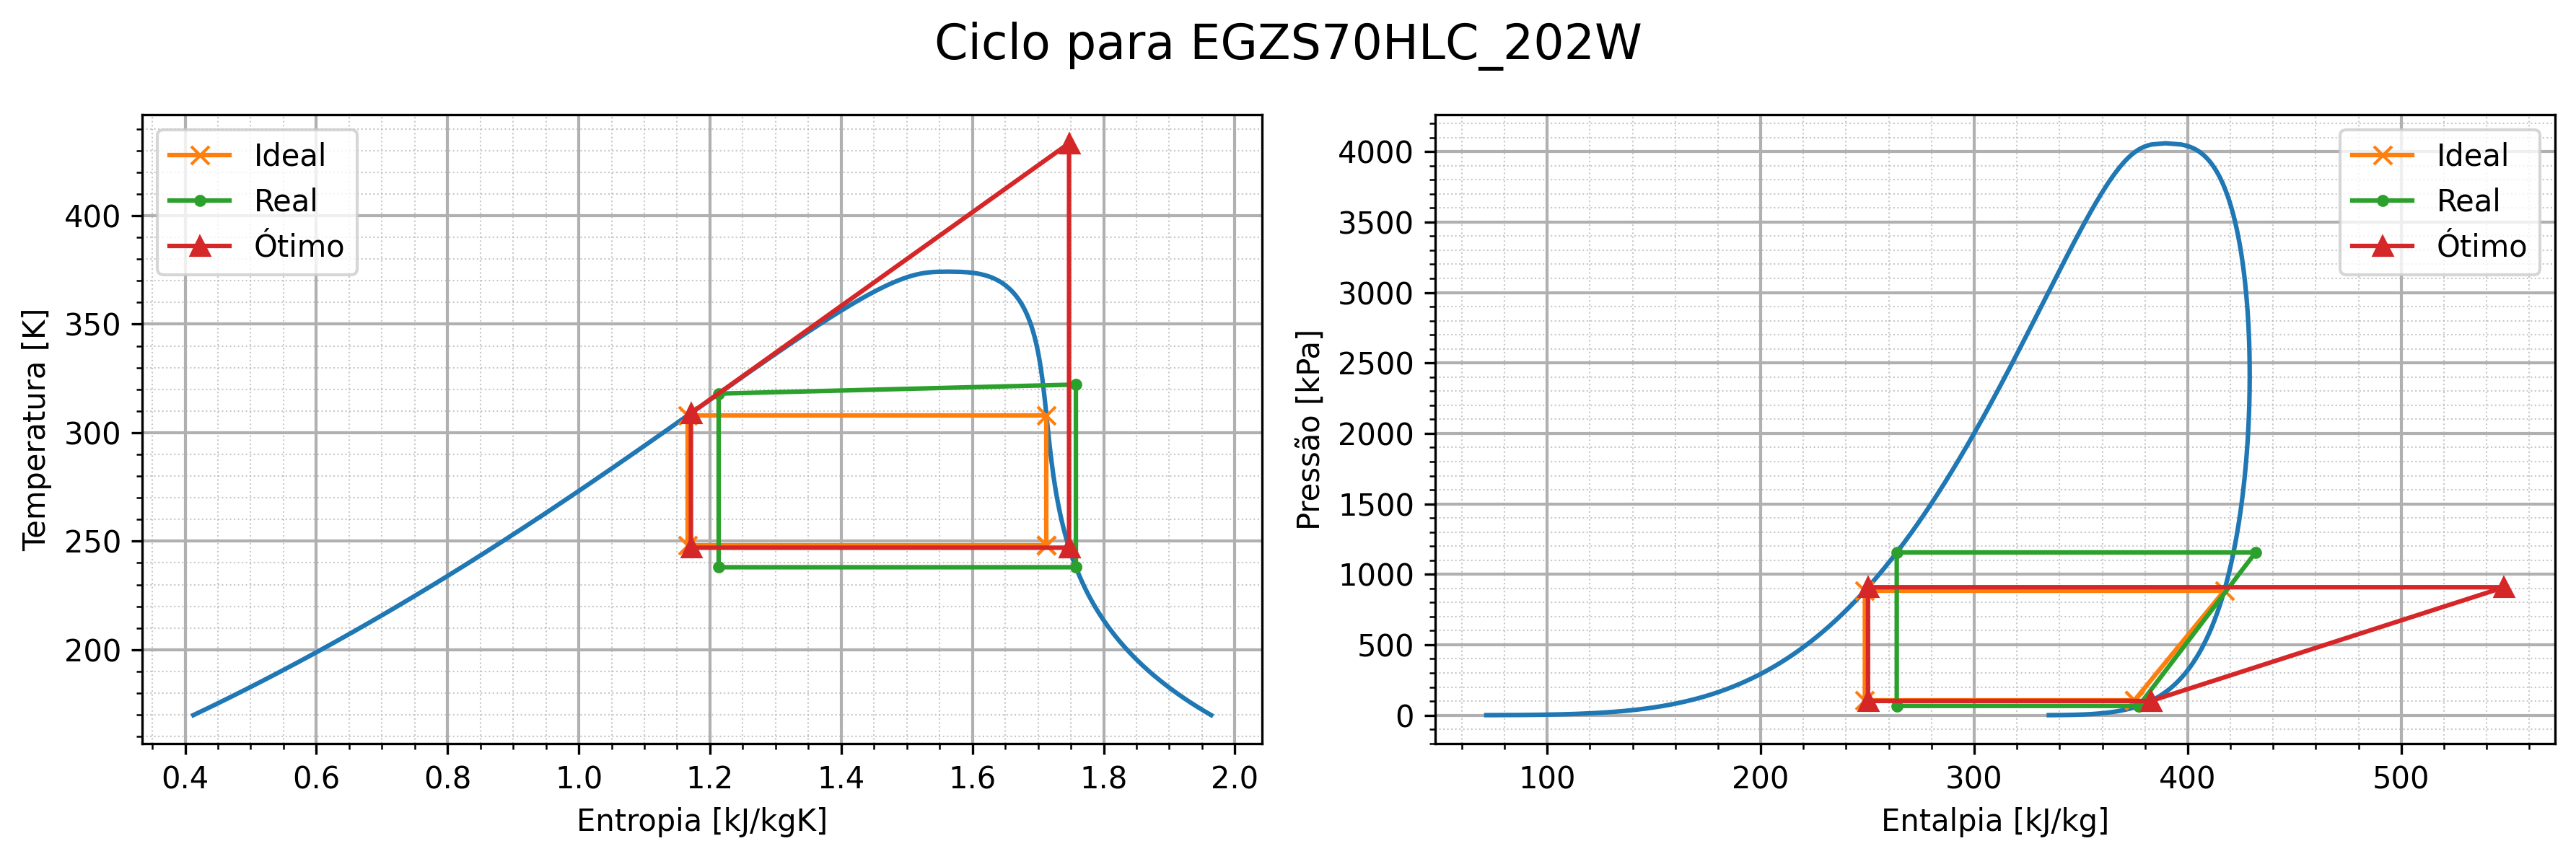
\includegraphics[width=\linewidth]{Imagens/Desenvolvimento/ciclo_EGZS70HLC_202W.png}
    \caption{Ciclo para o EGZS70HLC.}
    \label{fig:ciclo comp 1}
\end{figure}
Apenas os compressores \ref{fig:ciclo comp 1} e \ref{fig:ciclo comp 2} convergiram a resultados aceitáveis, gerando dúvidas no método utilizado.


\begin{figure}[ht]
    \centering
    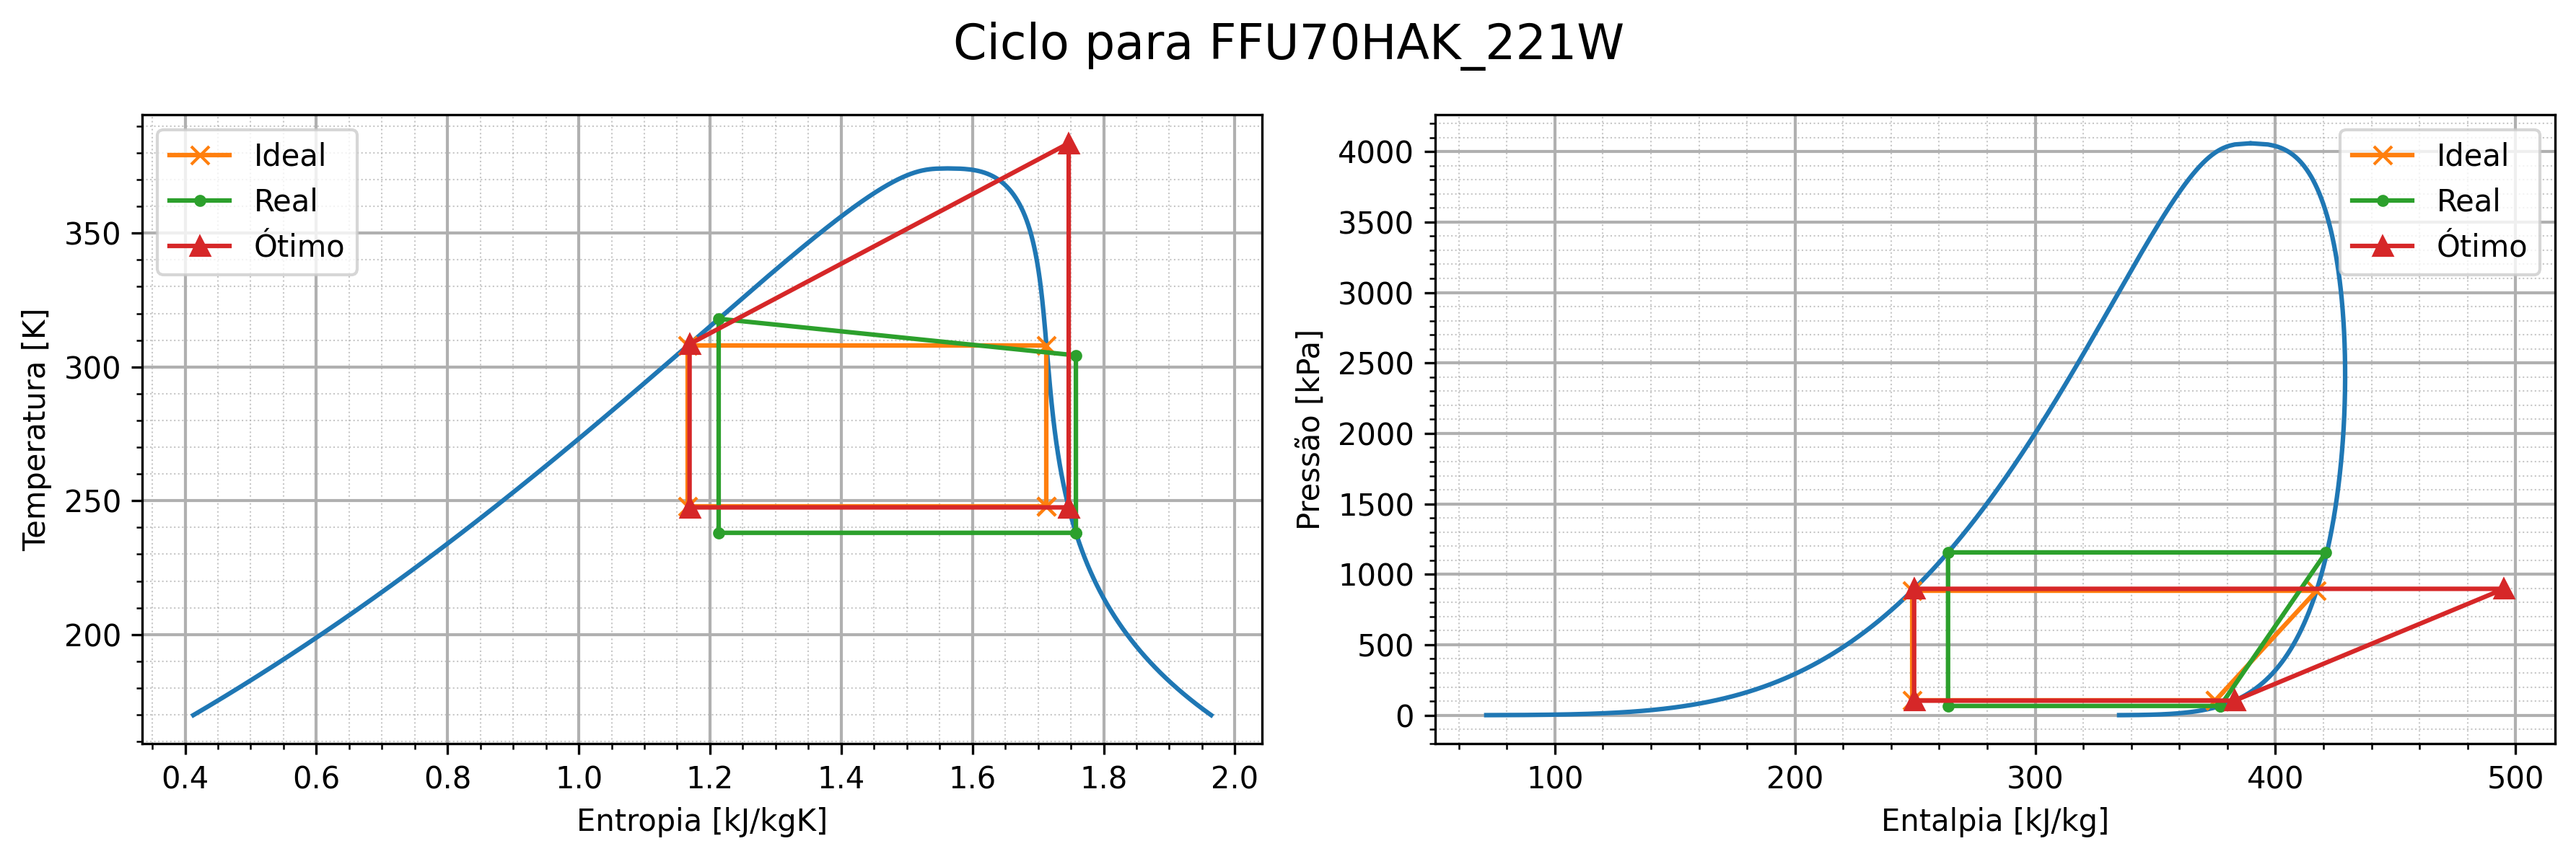
\includegraphics[width=\linewidth]{Imagens/Desenvolvimento/ciclo_FFU70HAK_221W.png}
    \caption{Ciclo para o FFU70HAK.}
    \label{fig:ciclo comp 2}
\end{figure}



Foi desenvolvida uma rotina de otimização utilizando a ferramenta \textit{Minimize} do pacote \textit{Scipy}, que foi utilizado para variar as temperaturas do condensador e do compressor a fim de minimizar o gasto energético, identificando a maior eficiência. Infelizmente os resultados não foram como esperado, resultando em temperatura muito similares com o ciclo de Carnot, porém com eficiência muito baixas, os resultados obtidos estão com a legenda "ótimo".

Nota-se que o compressor FFU70HAK não possui nenhum conjunto de temperaturas presente no banco de dados que satisfaça a condição da temperatura no início do condensador ser maior que no final, invalidando o ciclo.

A análise comparativa entre os diferentes ciclos revela diferenças significativas nos parâmetros de desempenho. A rotina computacional desenvolvida calcula sistematicamente a vazão mássica de refrigerante ($\dot{m}$), potência de compressão ($\dot{W}_c$), coeficiente de performance (COP) e capacidade de refrigeração ($\dot{Q}_L$) para os ciclos real e otimizado com dados de catálogo e otimizado, conforme apresentado nas Figuras~\ref{fig:barras fluxo massa} a~\ref{fig:barras Ql}.

\begin{figure}[ht]
    \centering
    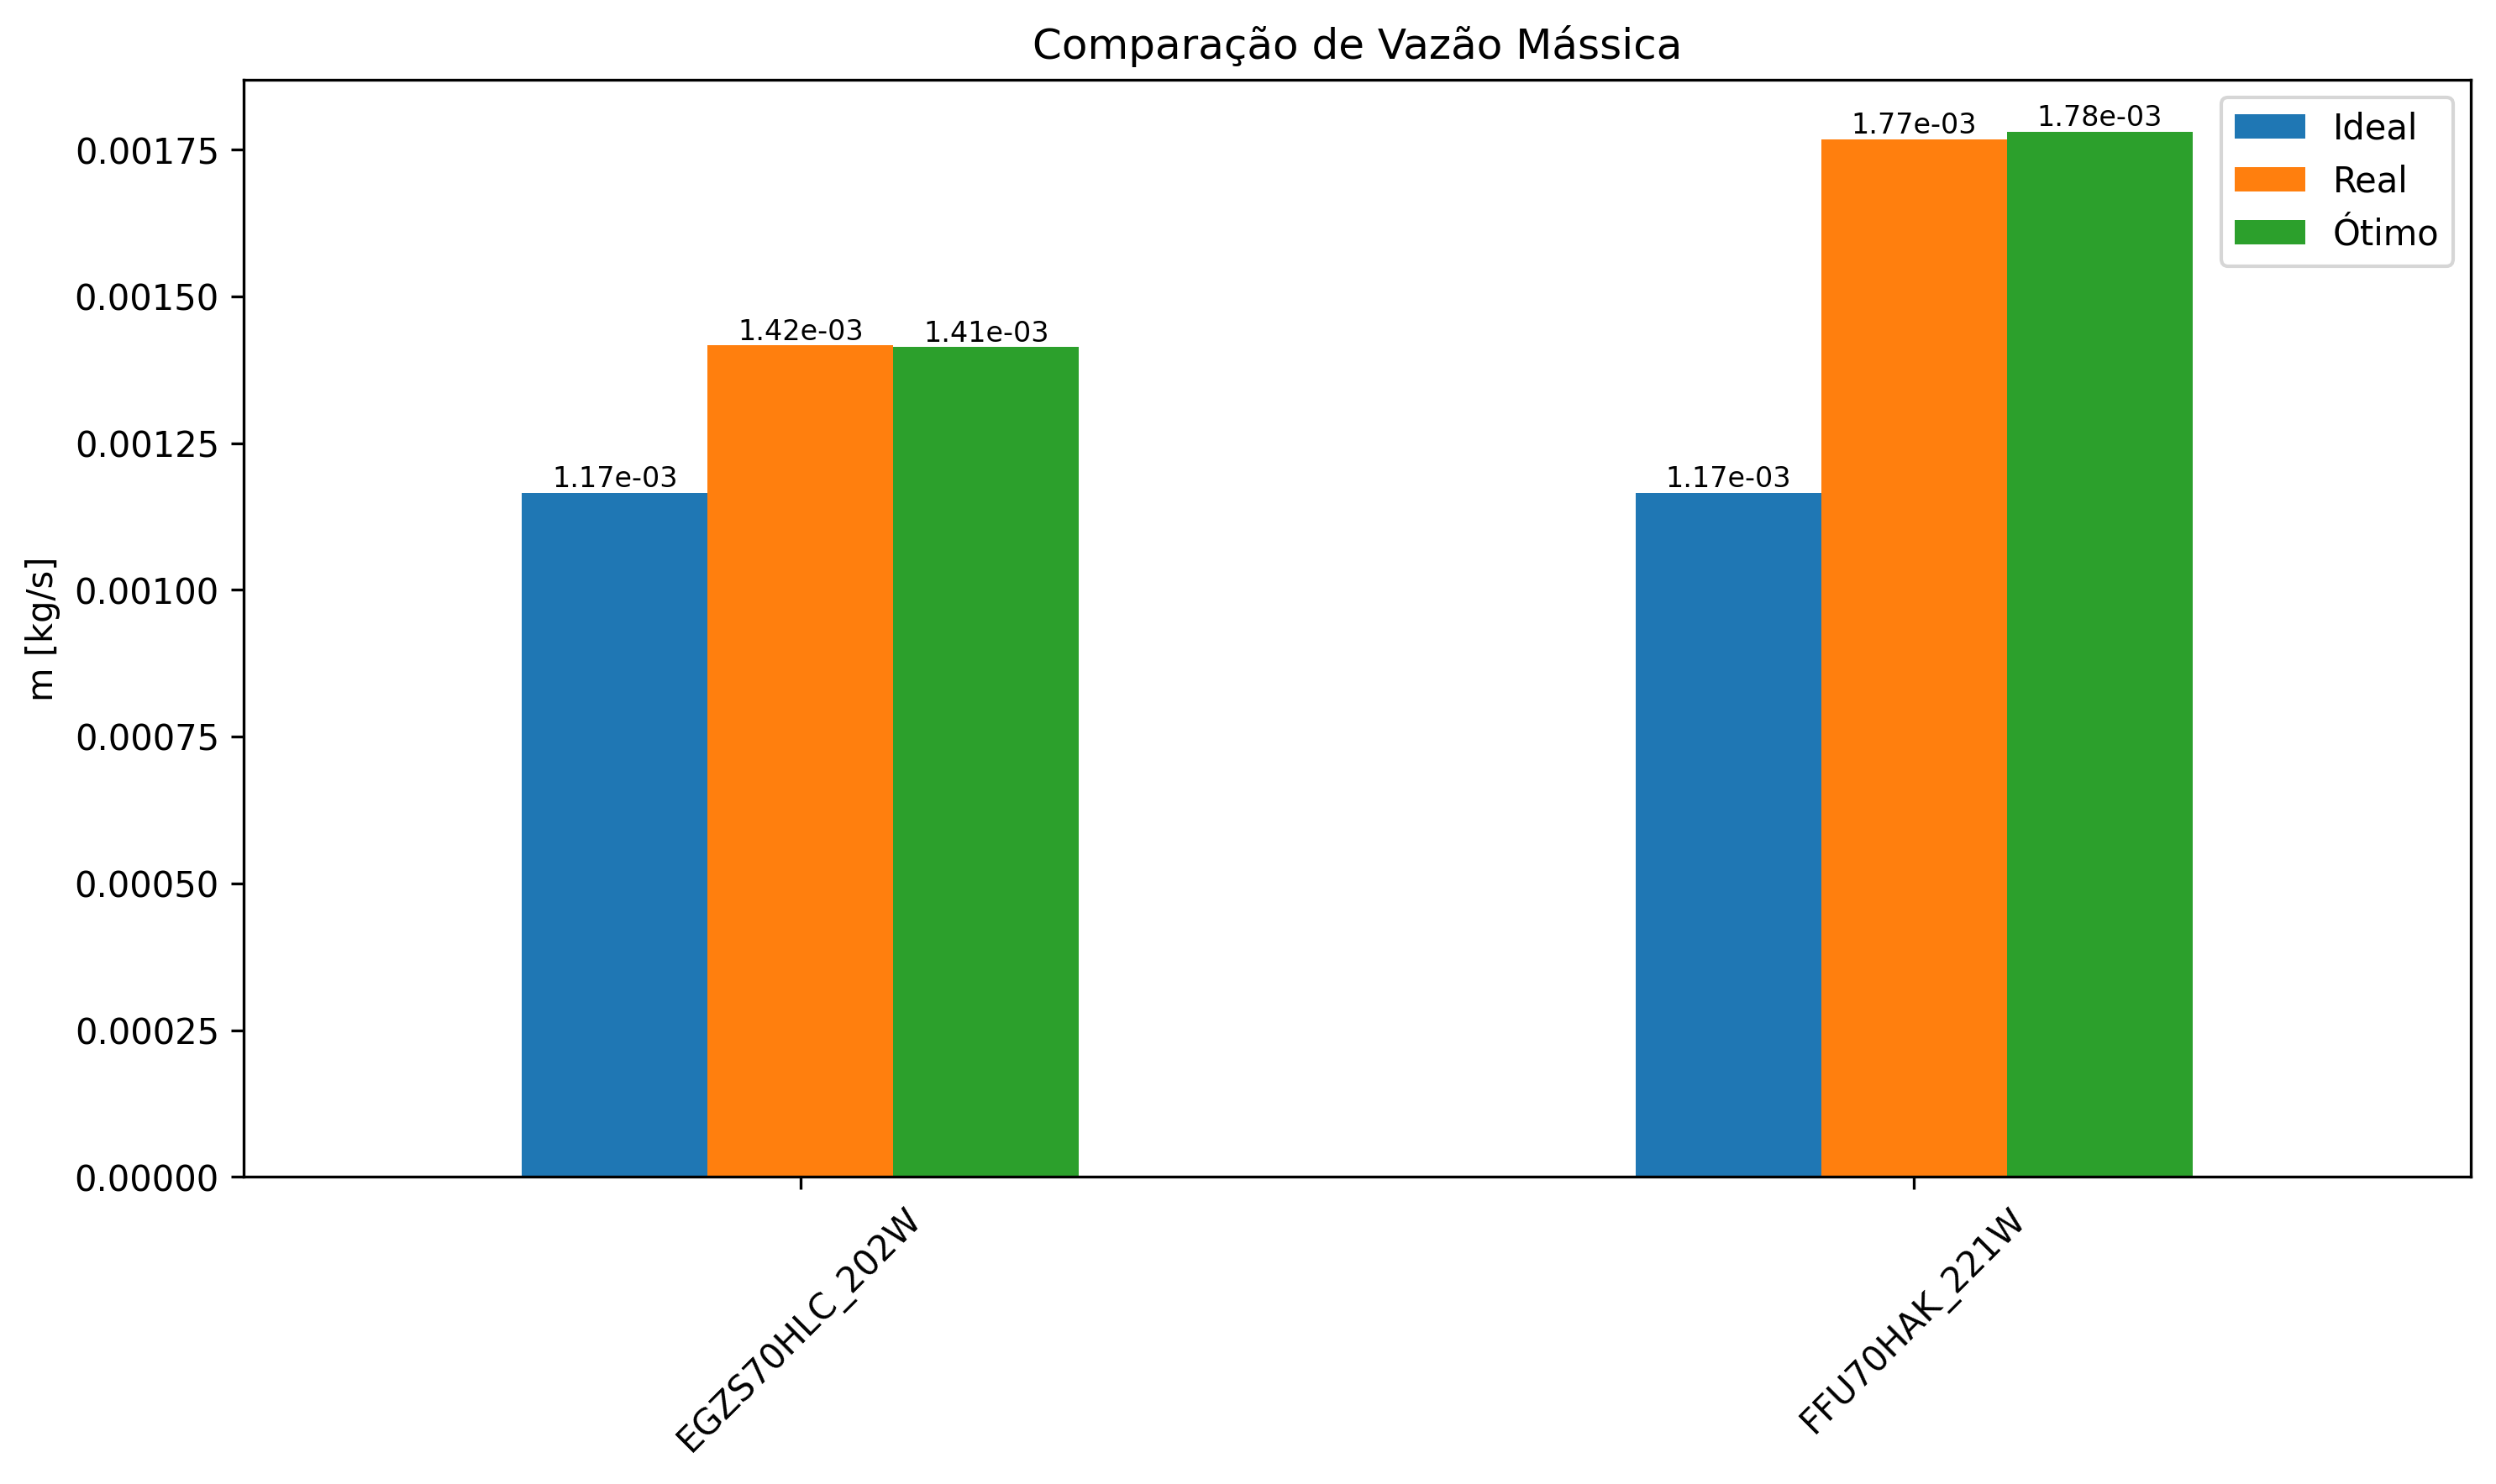
\includegraphics[width=0.8\linewidth]{Imagens/Desenvolvimento/barras_m.png}
    \caption{Comparação da vazão mássica de refrigerante entre os ciclos ideal, real e otimizado para os compressores selecionados.}
    \label{fig:barras fluxo massa}
\end{figure}

\begin{figure}[ht]
    \centering
    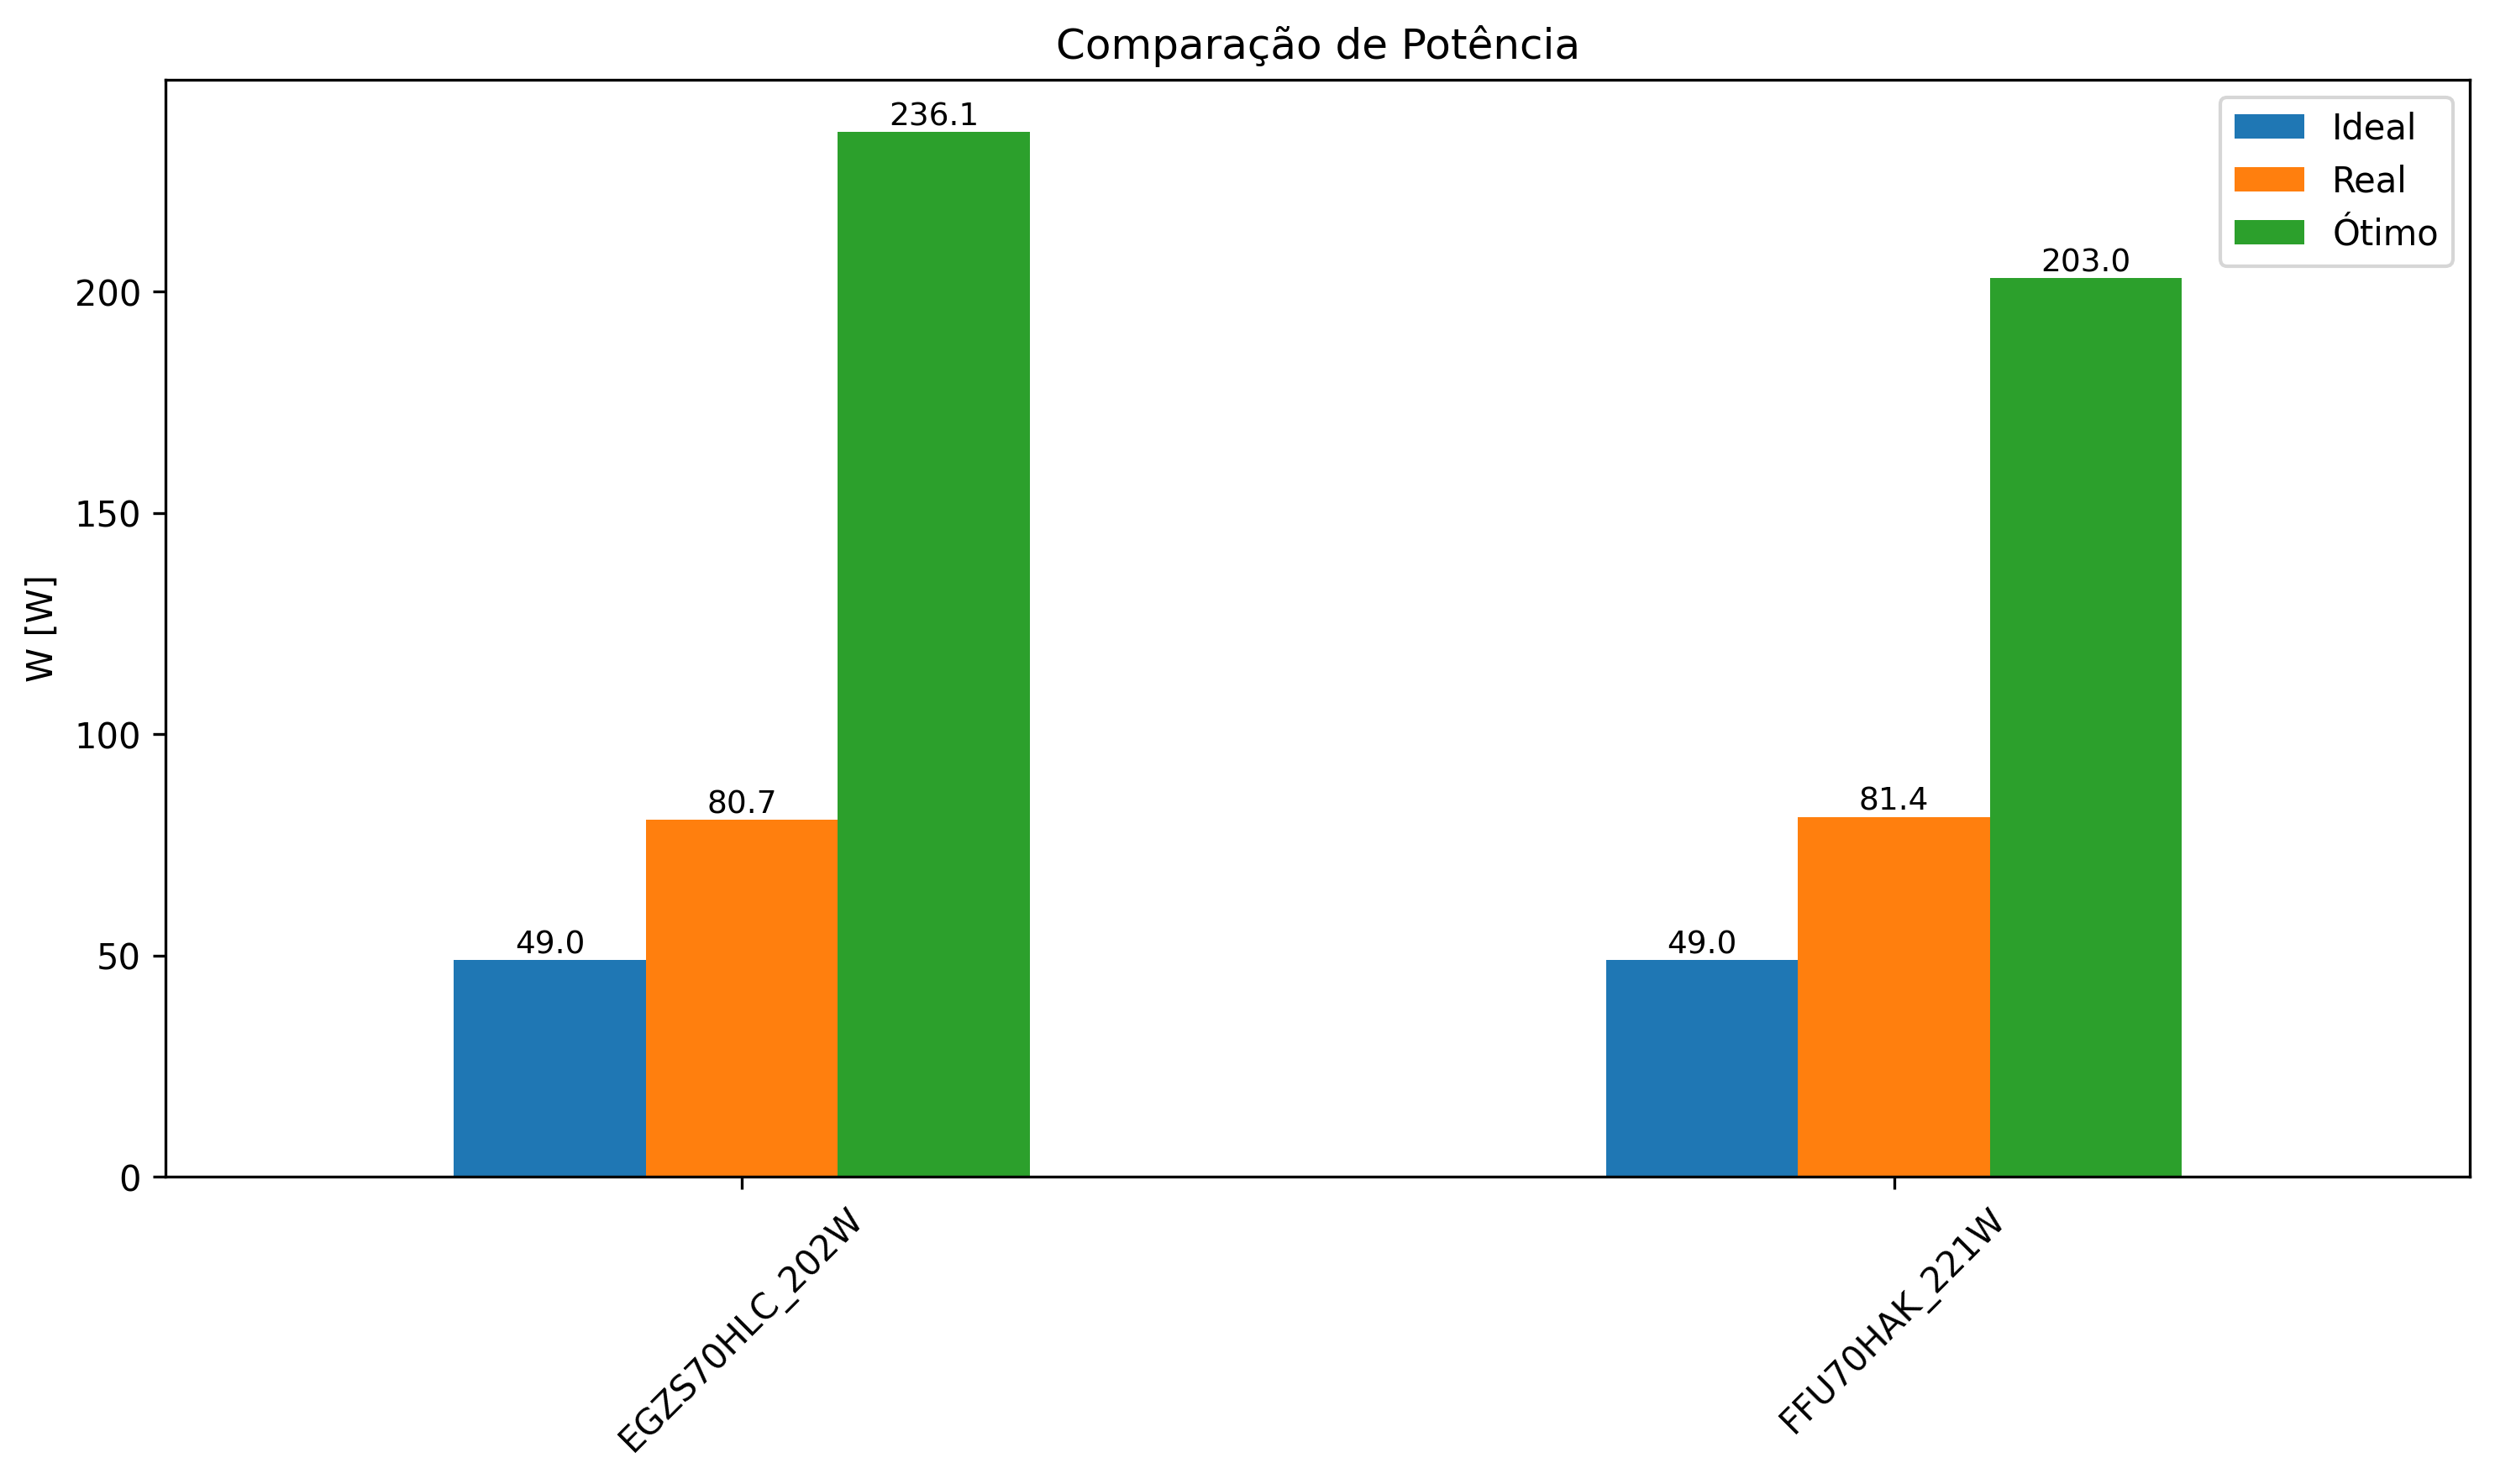
\includegraphics[width=0.8\linewidth]{Imagens/Desenvolvimento/barras_W.png}
    \caption{Comparação da potência de compressão entre os ciclos analisados.}
    \label{fig:barras W}
\end{figure}

\begin{figure}[ht]
    \centering
    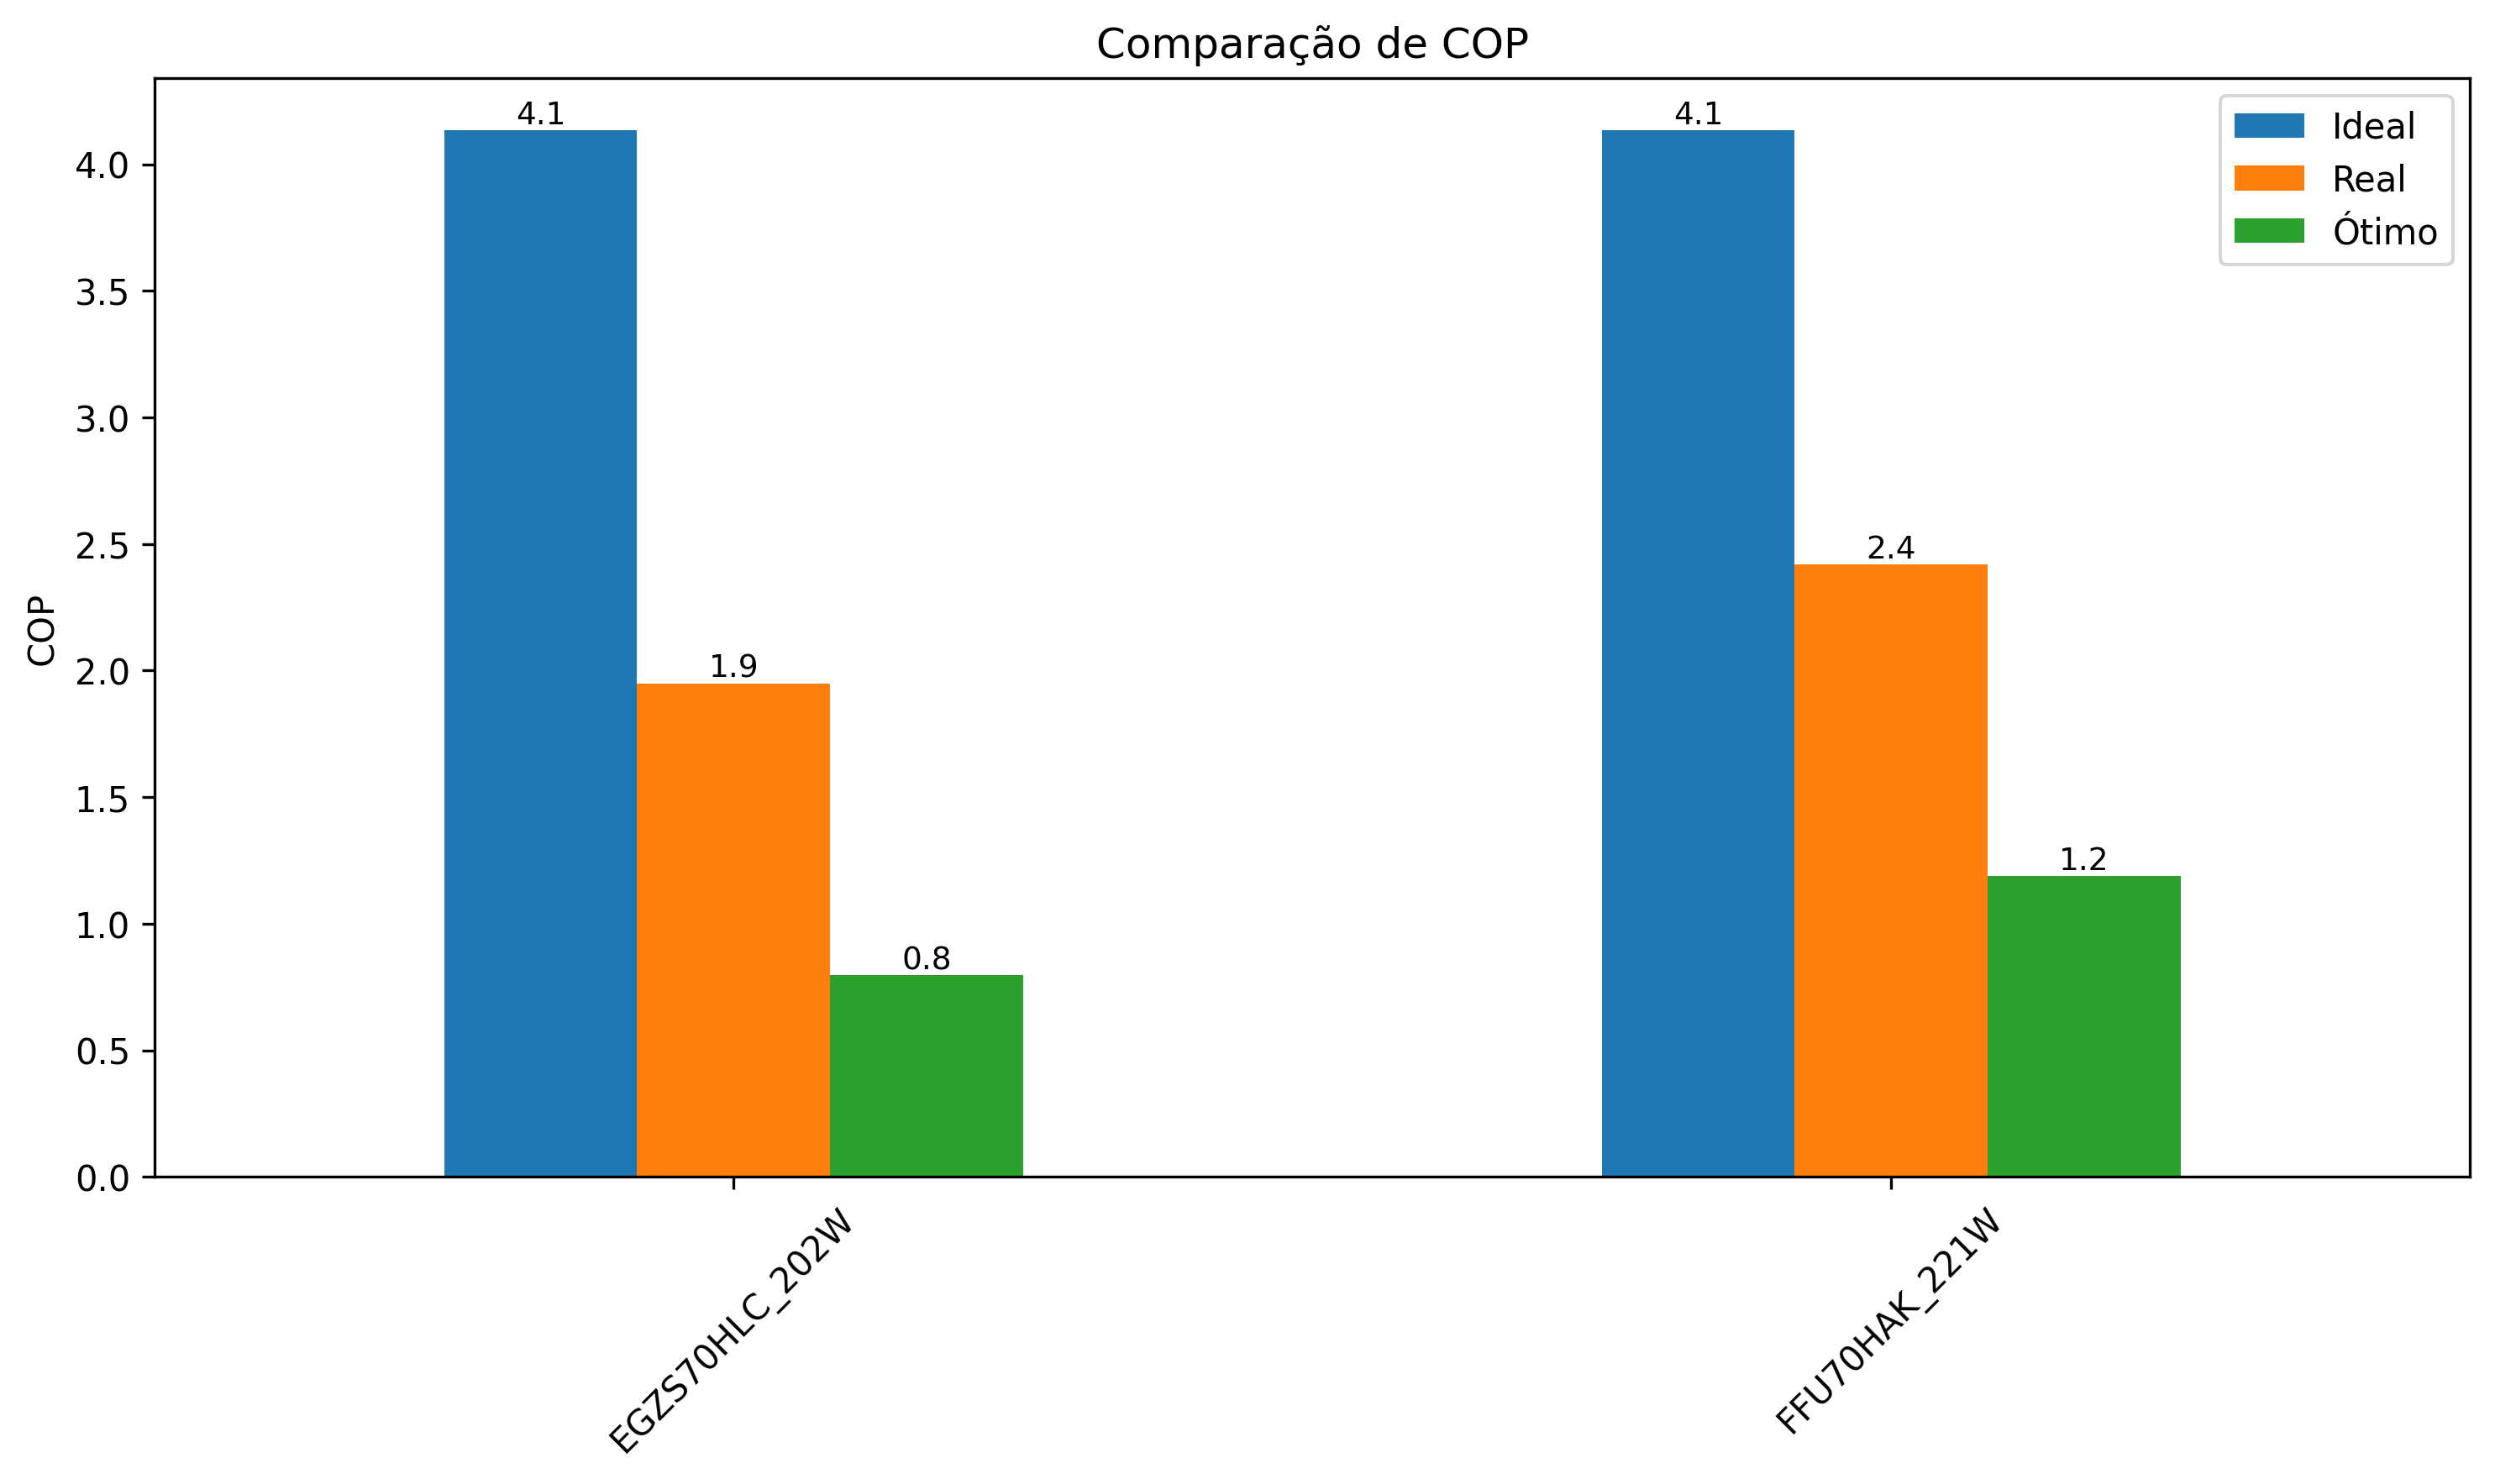
\includegraphics[width=0.8\linewidth]{Imagens/Desenvolvimento/barras_COP.png}
    \caption{Comparação do coeficiente de performance (COP) entre os diferentes ciclos.}
    \label{fig:barras COP}
\end{figure}

\begin{figure}[ht]
    \centering
    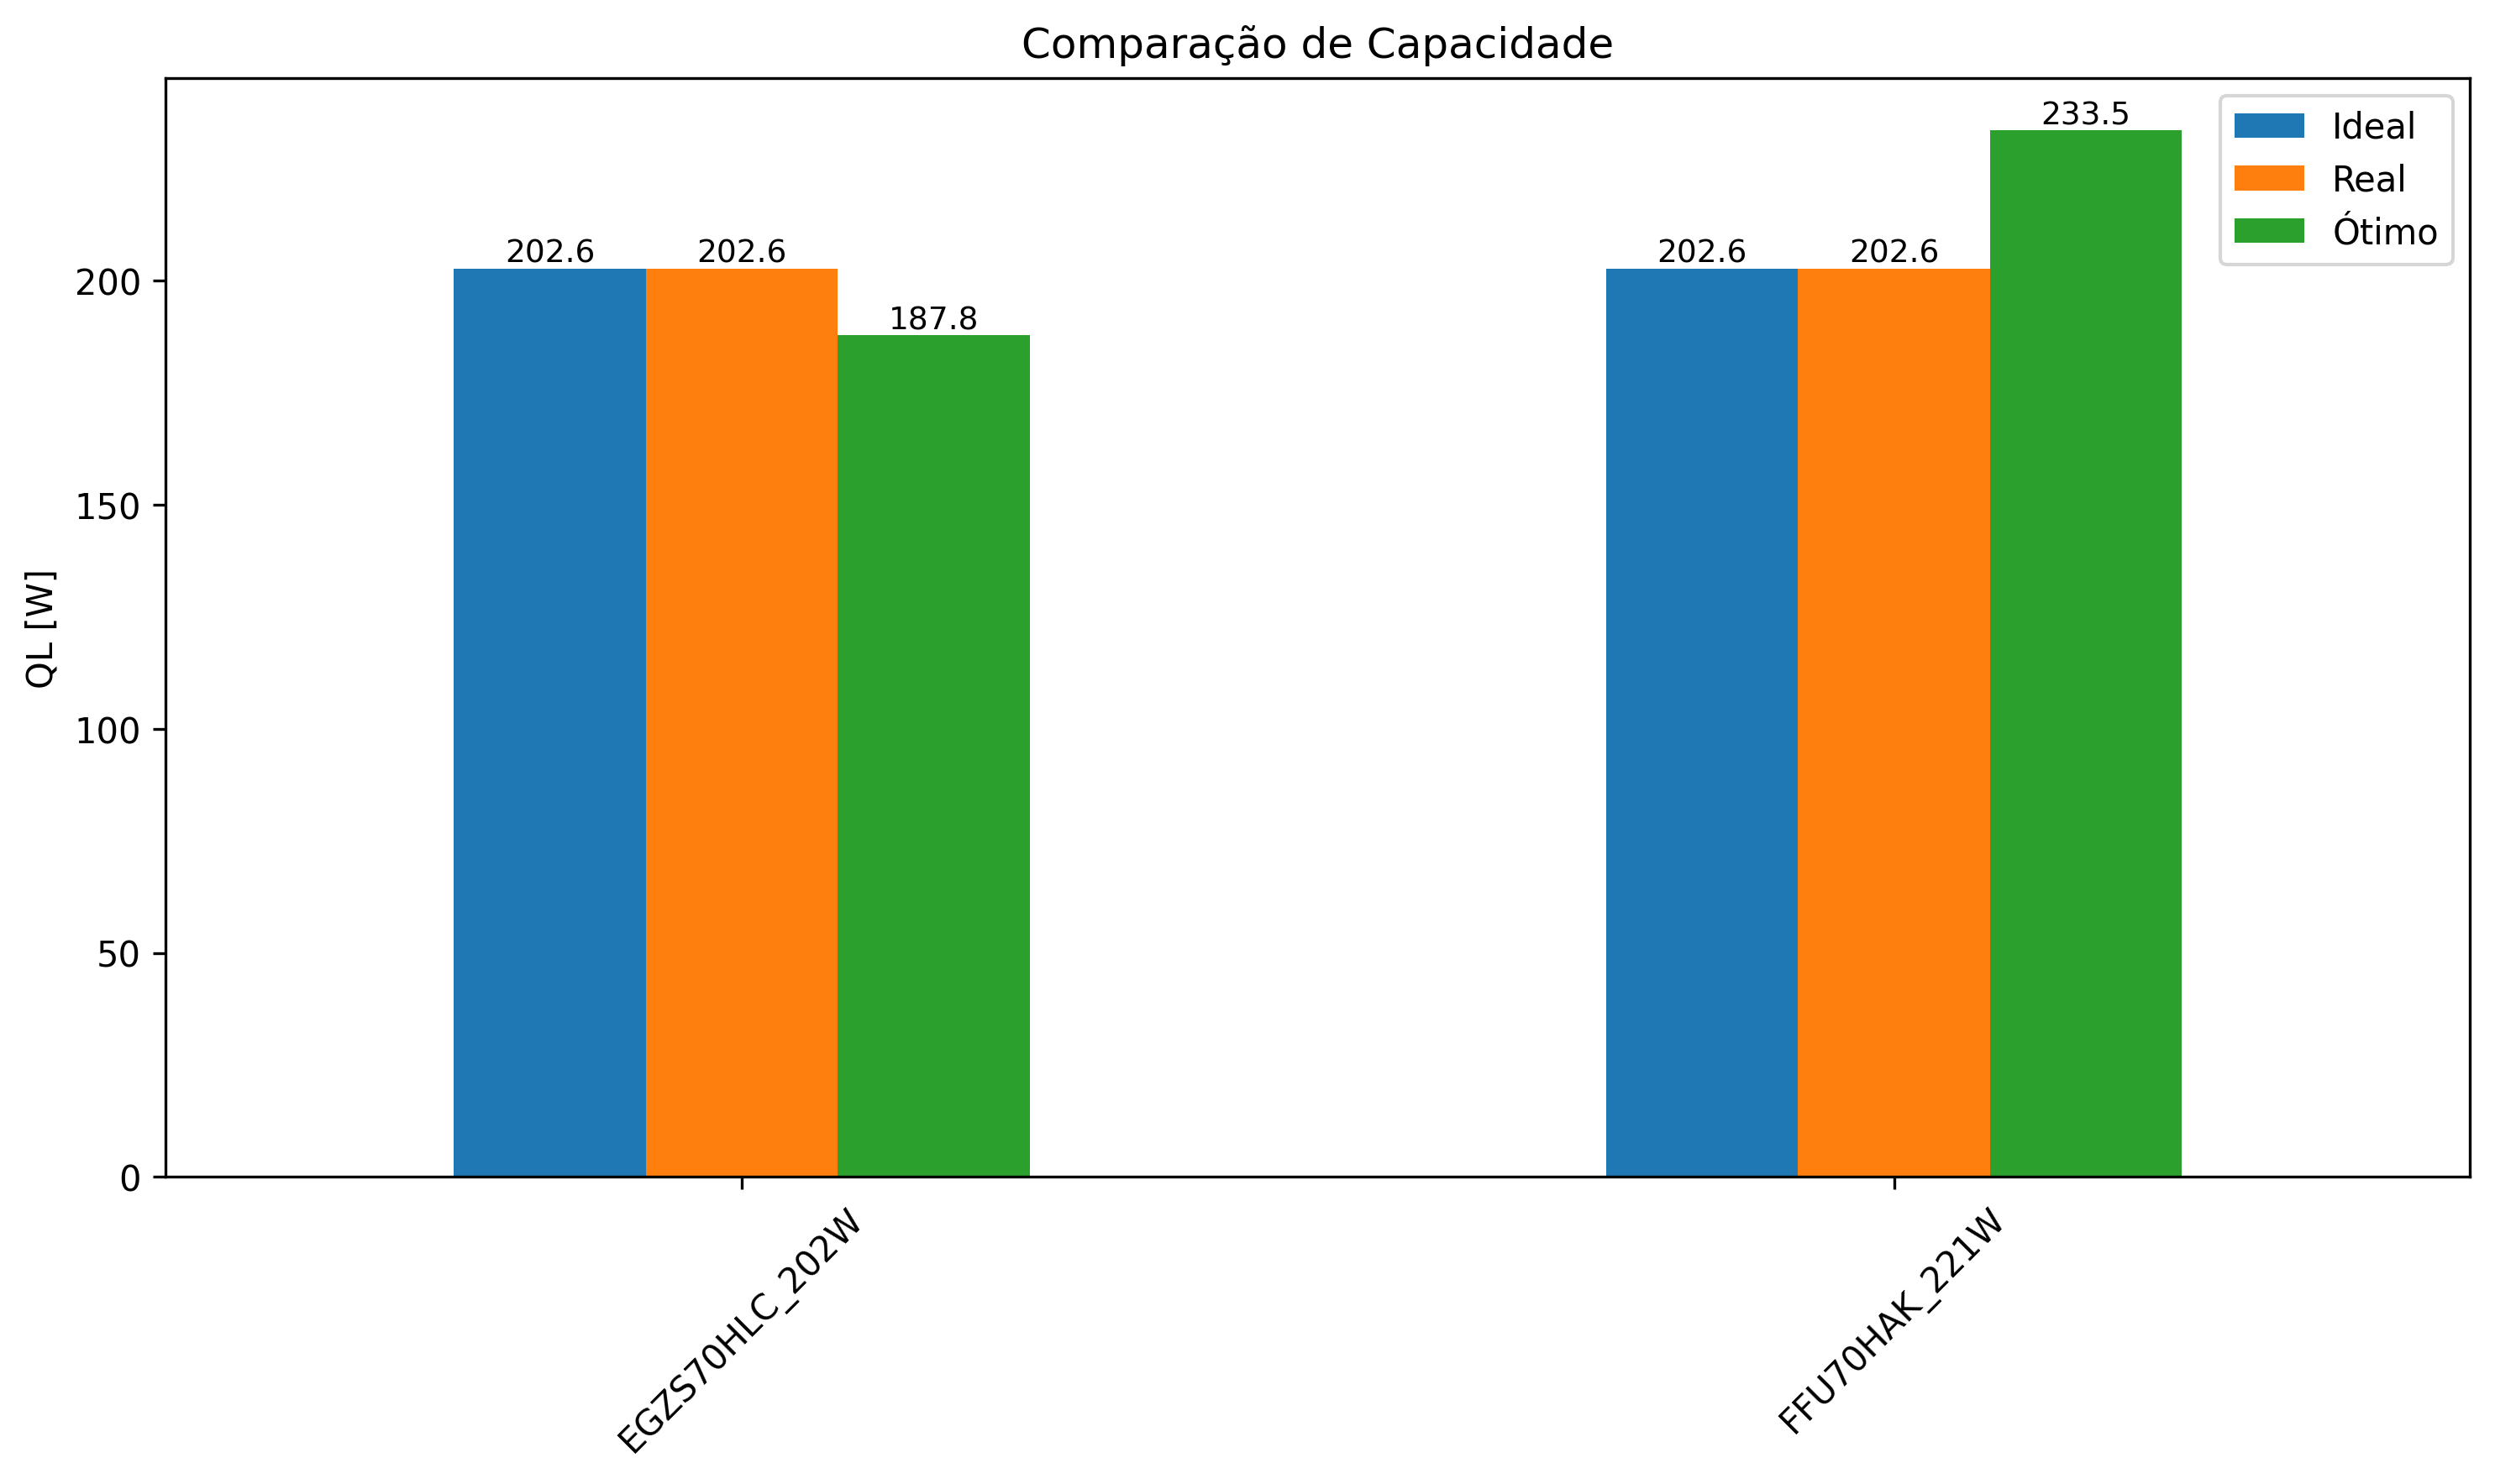
\includegraphics[width=0.8\linewidth]{Imagens/Desenvolvimento/barras_QL.png}
    \caption{Comparação da capacidade de refrigeração entre os ciclos estudados.}
    \label{fig:barras Ql}
\end{figure}

\subsection{Análise dos Resultados}

Os resultados apresentados nas Figuras~\ref{fig:barras fluxo massa} a~\ref{fig:barras Ql} demonstram comportamento coerente com a teoria termodinâmica de ciclos de refrigeração, permitindo identificar o impacto das irreversibilidades nos parâmetros de desempenho:

\textbf{Vazão mássica ($\dot{m}$):} O ciclo ideal de Carnot apresenta a menor vazão mássica necessária, uma vez que opera com a máxima eficiência termodinâmica possível. Os ciclos real e otimizado requerem vazões superiores para fornecer a mesma capacidade de refrigeração, compensando as perdas por irreversibilidades, como expansão isentálpica, superaquecimento do vapor na descarga do compressor e diferenças finitas de temperatura nos trocadores de calor.

\textbf{Coeficiente de Performance (COP):} O ciclo de Carnot estabelece o limite superior teórico de eficiência, servindo como referencial para avaliar o desempenho dos ciclos reais. A diferença entre o COP de Carnot e o COP real quantifica o efeito combinado de todas as irreversibilidades presentes no sistema.

\textbf{Potência de compressão ($\dot{W}_c$):} O ciclo ideal requer a menor potência de compressão devido à sua máxima eficiência. O ciclo real demanda potência significativamente superior devido às perdas já mencionadas, enquanto o ciclo otimizado busca um compromisso entre capacidade de refrigeração e consumo energético através da seleção apropriada das condições operacionais.

\textbf{Capacidade de refrigeração ($\dot{Q}_L$):} Observa-se que os diferentes ciclos fornecem capacidades de refrigeração distintas devido às variações na eficiência volumétrica do compressor e no efeito refrigerante específico, influenciados pelas condições de evaporação e condensação adotadas.

A Tabela~\ref{tab:eficiencias termo} apresenta as eficiências termodinâmicas calculadas para dois dos compressores analisados, tanto nas condições reais de catálogo quanto nas condições otimizadas. A eficiência $\eta_{II}$ representa a razão entre o COP real e otimizado em relação ao COP de Carnot, indicando o quão próximo o sistema opera do limite termodinâmico ideal.

\begin{table}[ht]
\centering
\begin{tabular}{|l|c|c|}
\hline
\textbf{Modelo} & \textbf{$\eta_{II}$ Real [\%]} & \textbf{$\eta_{II}$ Otimizado [\%]} \\ \hline
EGZS70HLC & 46,3 & 29,2 \\ \hline
FFU70HAK & 58,5 & 19,5 \\ \hline
\end{tabular}
\caption{Eficiências termodinâmicasdos compressores nas condições real e otimizada.}
\label{tab:eficiencias termo}
\end{table}

Observa-se que as eficiências termodinâmicas situam-se na faixa de 19,5\% a 58,5\%, valores típicos para sistemas de refrigeração operando com elevadas razões de compressão. A redução da eficiência no ciclo otimizado em relação ao ciclo real deve-se a interpolação do banco de dados do fabricante, talvez representando melhor um ciclo real.

\section{Análise de Geração de Entropia e Potência Perdida}

A análise de irreversibilidades através da geração de entropia permite quantificar as perdas termodinâmicas em cada componente do sistema de refrigeração e identificar oportunidades de melhoria no desempenho energético. Esta seção apresenta os cálculos de geração de entropia e potência perdida para o evaporador e condensador, considerando as condições operacionais do ciclo otimizado.

\subsection{Condições Operacionais Analisadas}

A análise foi realizada para as seguintes condições de operação:

\begin{itemize}
    \item Temperatura de evaporação: $T_e = -30$°C (243 K)
    \item Temperatura de condensação: $T_c = 40$°C (313 K)
    \item Vazão mássica de refrigerante: $\dot{m} = 0{,}000792$ kg/s
    \item Capacidade frigorífica: $\dot{Q}_L = 186$ W
    \item Potência de compressão: $\dot{W}_c = 160$ W
    \item Calor rejeitado no condensador: $\dot{Q}_H = \dot{Q}_L + \dot{W}_c = 346$ W
\end{itemize}

As temperaturas do produto refrigerado e do ambiente externo foram consideradas como $T_1 = -25$°C com diferença de temperatura de $\Delta T_1 = -5$°C no evaporador, e $T_3 = 35$°C com $\Delta T_3 = +5$°C no condensador, resultando nas temperaturas de evaporação e condensação especificadas.

\subsection{Propriedades Termodinâmicas do Refrigerante}

As entropias específicas do R-134a nos estados principais do ciclo foram determinadas através da biblioteca CoolProp:

\begin{table}[ht]
\centering
\begin{tabular}{|c|c|c|}
\hline
\textbf{Estado} & \textbf{Descrição} & \textbf{Entropia [J/(kg·K)]} \\ \hline
1 & Entrada do compressor (vapor saturado) & 1757,72 \\ \hline
2 & Saída do compressor (vapor superaquecido) & 1757,72 \\ \hline
3 & Saída do condensador (líquido saturado) & 1213,24 \\ \hline
4 & Saída da válvula de expansão & 1213,24 \\ \hline
\end{tabular}
\caption{Entropias específicas do R-134a nos estados do ciclo de refrigeração.}
\label{tab:entropias}
\end{table}

Observa-se que $s_2 = s_1$, confirmando a hipótese de compressão isentrópica, e $s_4 = s_3$, indicando o processo de expansão isentálpica através do dispositivo de expansão.

\subsection{Cálculo da Geração de Entropia}

\subsubsection{Evaporador}

A taxa de geração de entropia no evaporador foi calculada através do balanço de entropia, considerando a transferência de calor com o ambiente refrigerado a $-30$°C:

\begin{equation}
    \dot{S}_{\text{ger,evap}} = \dot{m}(s_1 - s_4) + \frac{\dot{Q}_L}{T_{\text{ext,evap}}}
\end{equation}

Substituindo os valores:

\begin{equation}
    \dot{S}_{\text{ger,evap}} = 0{,}000792 \times (1757{,}72 - 1213{,}24) + \frac{186}{243}
\end{equation}

\begin{equation}
    \dot{S}_{\text{ger,evap}} = 0{,}431 + 0{,}765 = 1{,}196~\text{W/K}
\end{equation}

A potência perdida associada à irreversibilidade no evaporador é:

\begin{equation}
    \dot{W}_{\text{perdida,evap}} = T_e \cdot \dot{m} \cdot \dot{S}_{\text{ger,evap}} = 243 \times 0{,}000792 \times 1{,}196 = 0{,}230~\text{W}
\end{equation}

\subsubsection{Condensador}

Para o condensador, a geração de entropia considera a rejeição de calor para o ambiente externo a $40$°C:

\begin{equation}
    \dot{S}_{\text{ger,cond}} = \dot{m}(s_3 - s_2) + \frac{\dot{Q}_H}{T_{\text{ext,cond}}}
\end{equation}

Substituindo os valores:

\begin{equation}
    \dot{S}_{\text{ger,cond}} = 0{,}000792 \times (1213{,}24 - 1757{,}72) + \frac{346}{313}
\end{equation}

\begin{equation}
    \dot{S}_{\text{ger,cond}} = -0{,}431 + 1{,}105 = 0{,}674~\text{W/K}
\end{equation}

A potência perdida no condensador é:

\begin{equation}
    \dot{W}_{\text{perdida,cond}} = T_c \cdot \dot{m} \cdot \dot{S}_{\text{ger,cond}} = 313 \times 0{,}000792 \times 0{,}674 = 0{,}167~\text{W}
\end{equation}

\subsection{Síntese dos Resultados}

A Tabela~\ref{tab:geracao entropia} resume os resultados da análise de irreversibilidades:

\begin{table}[ht]
\centering
\begin{tabular}{|l|c|c|}
\hline
\textbf{Componente} & \textbf{Geração de Entropia [W/K]} & \textbf{Potência Perdida [W]} \\ \hline
Evaporador & 1,196 & 0,230 \\ \hline
Condensador & 0,674 & 0,167 \\ \hline
\textbf{Total} & \textbf{1,870} & \textbf{0,397} \\ \hline
\end{tabular}
\caption{Geração de entropia e potência perdida nos componentes do sistema.}
\label{tab:geracao entropia}
\end{table}

O evaporador apresenta maior taxa de geração de entropia (1,196 W/K) em comparação ao condensador (0,674 W/K), representando 64\% das irreversibilidades totais nos trocadores de calor. Isso indica que o evaporador constitui o principal ponto de perda termodinâmica do sistema, sugerindo que melhorias na transferência de calor ou redução da diferença de temperatura neste componente teriam maior impacto na eficiência global.

A potência perdida total de 0,397~W, embora relativamente pequena em relação à potência de compressão (160~W), representa trabalho adicional dissipado devido às irreversibilidades. O coeficiente de performance baseado nas temperaturas de evaporação e condensação é:

\begin{equation}
    \text{COP} = \frac{T_e}{T_c - T_e} = \frac{243}{313 - 243} = 3{,}47
\end{equation}

Este valor serve como referência para o desempenho termodinâmico esperado do sistema operando nas condições especificadas.